\newpage
\section{Anhang}

\subsection{Versuchsaufbauten}
\begin{figure}[H]
    \centering
    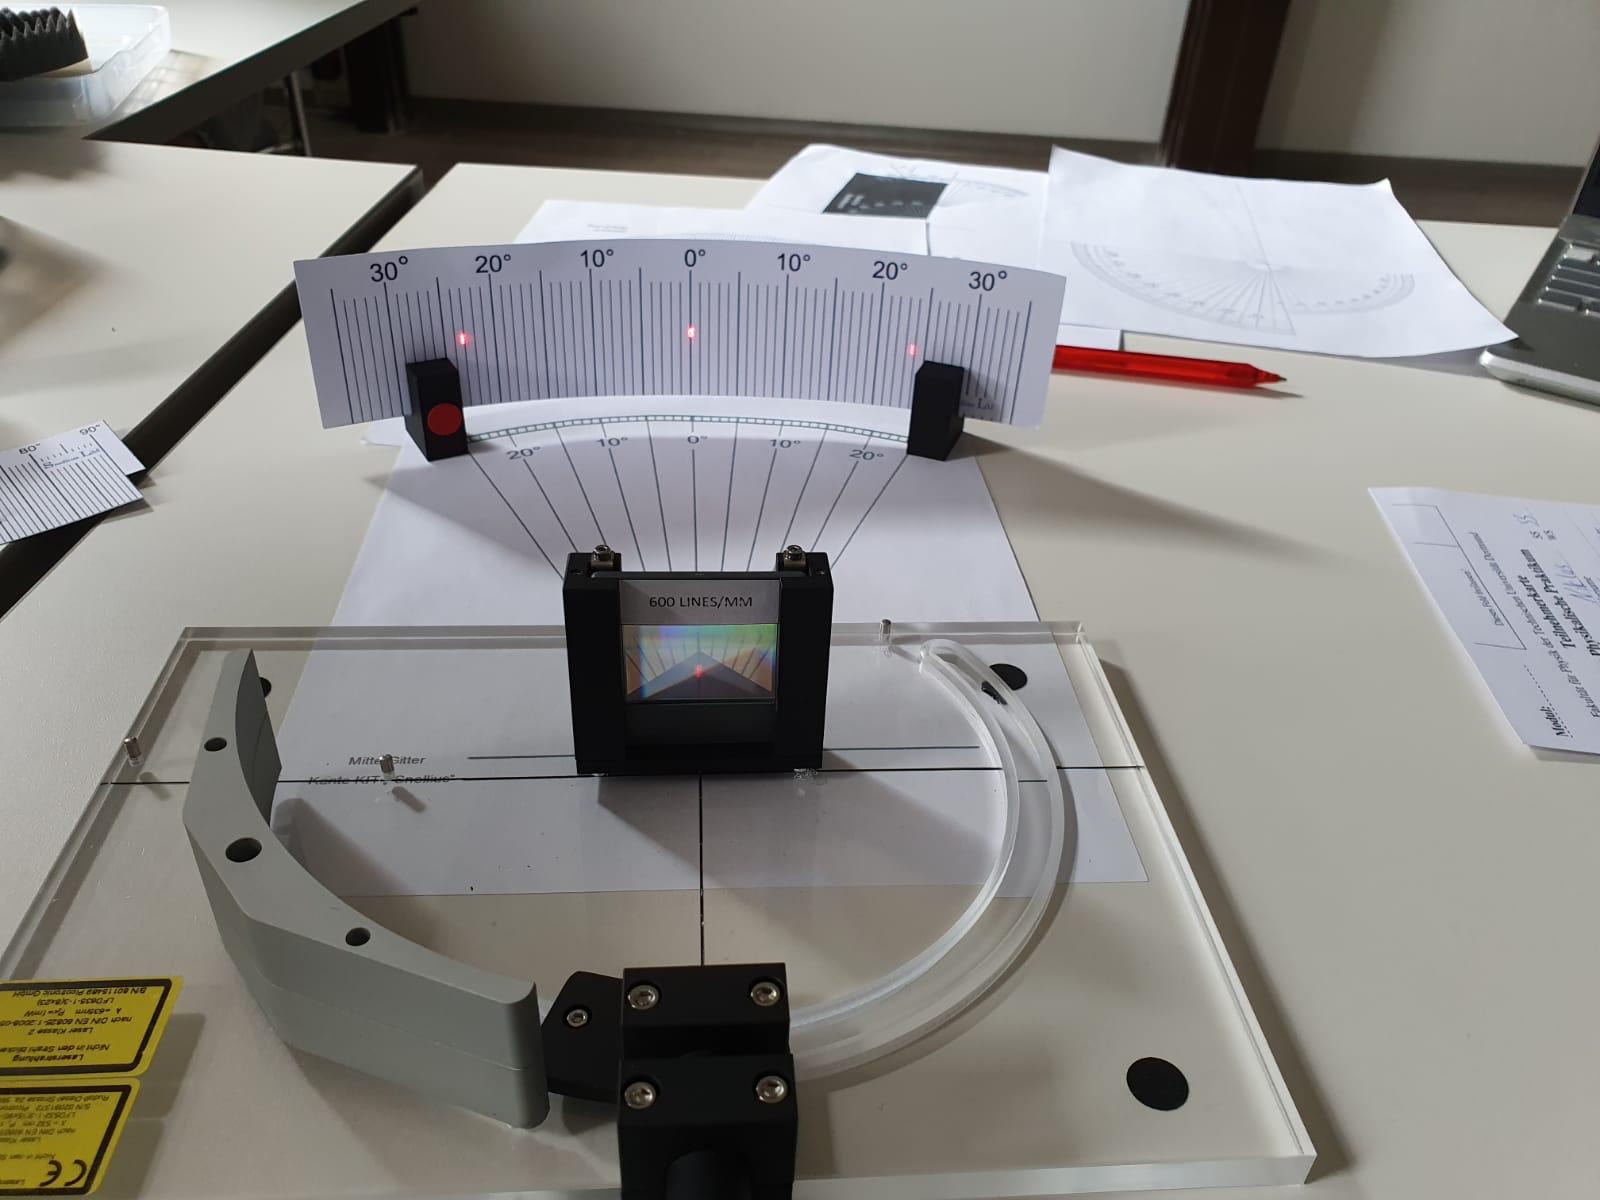
\includegraphics[width=0.63\textwidth]{latex/images/gitter.jpeg}
    \caption{Ein Foto des Aufbaus um Interferenz zu untersuchen.}
    \label{img:aufbaugitter}
\end{figure}

\begin{figure}[H]
    \centering
    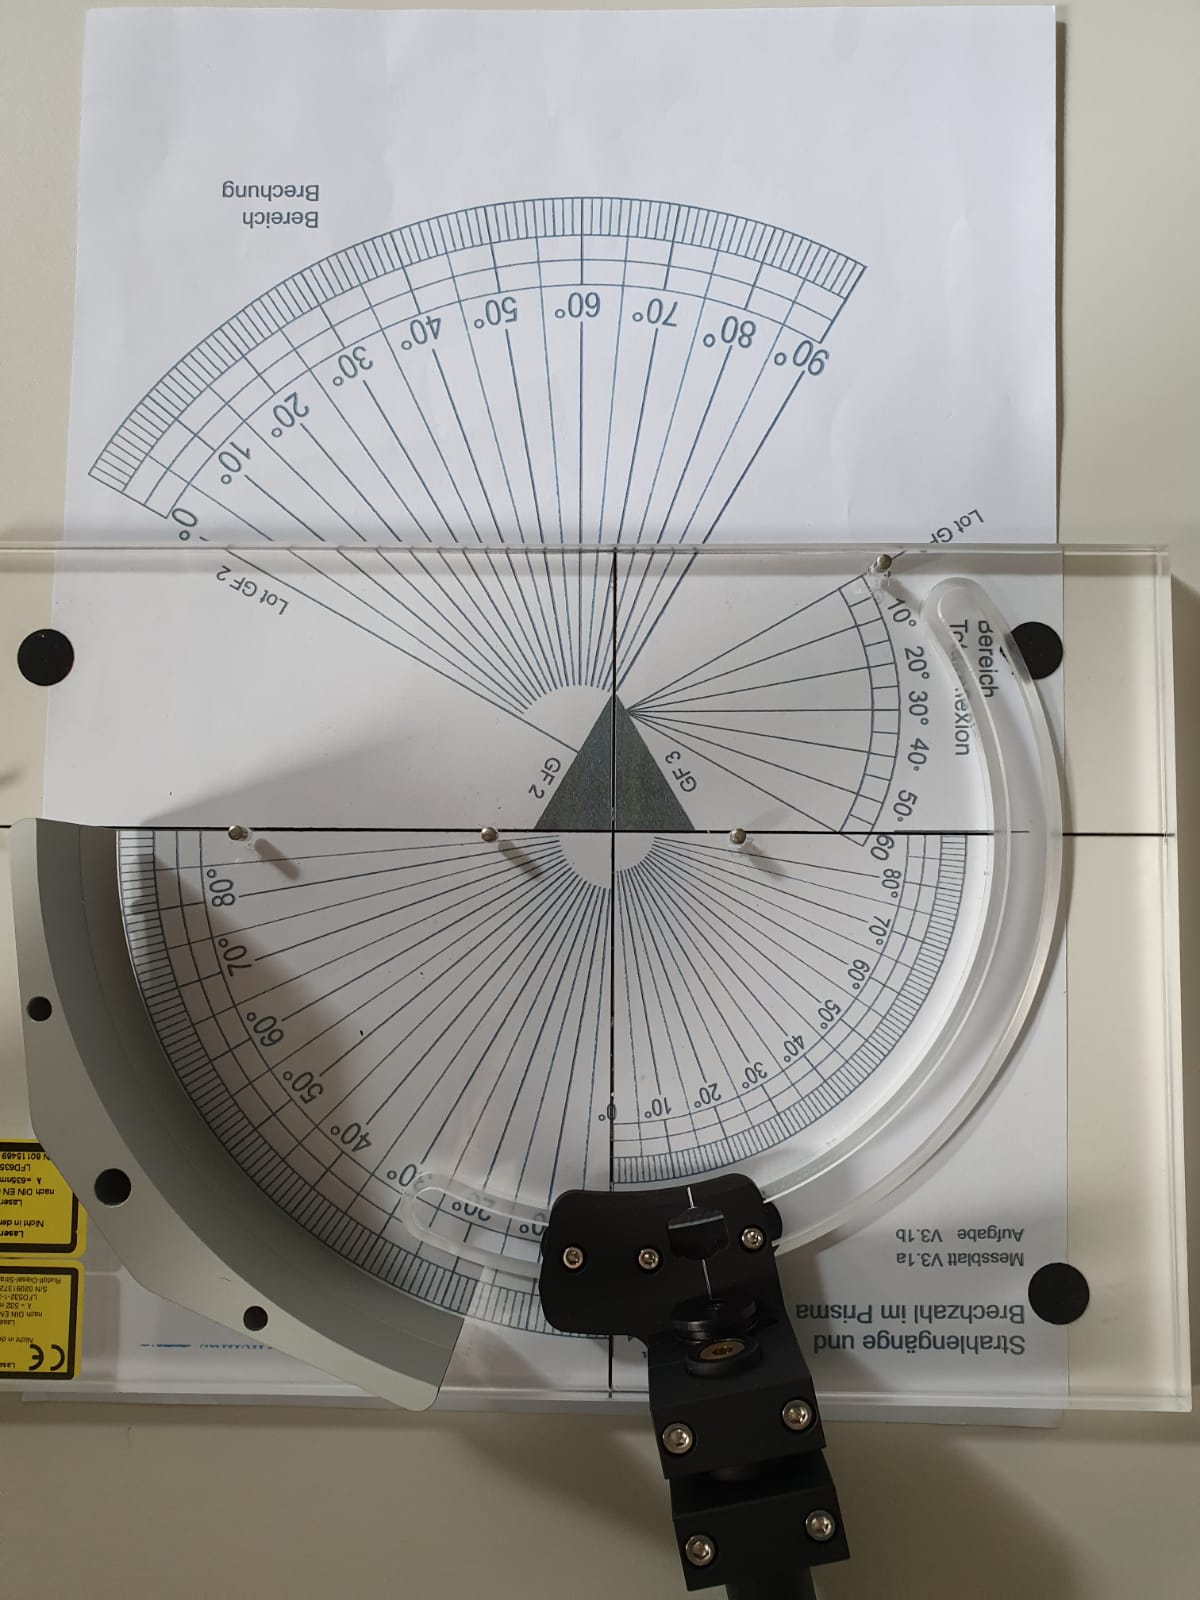
\includegraphics[width=0.63\textwidth]{latex/images/prisma.jpeg}
    \caption{Ein Foto des Aufbaus um die Brechung des Lichts an einem Prisma zu untersuchen.}
    \label{img:aufbauprisma}
\end{figure}


\subsection{Daten}
\begin{figure}[H]
    \centering
    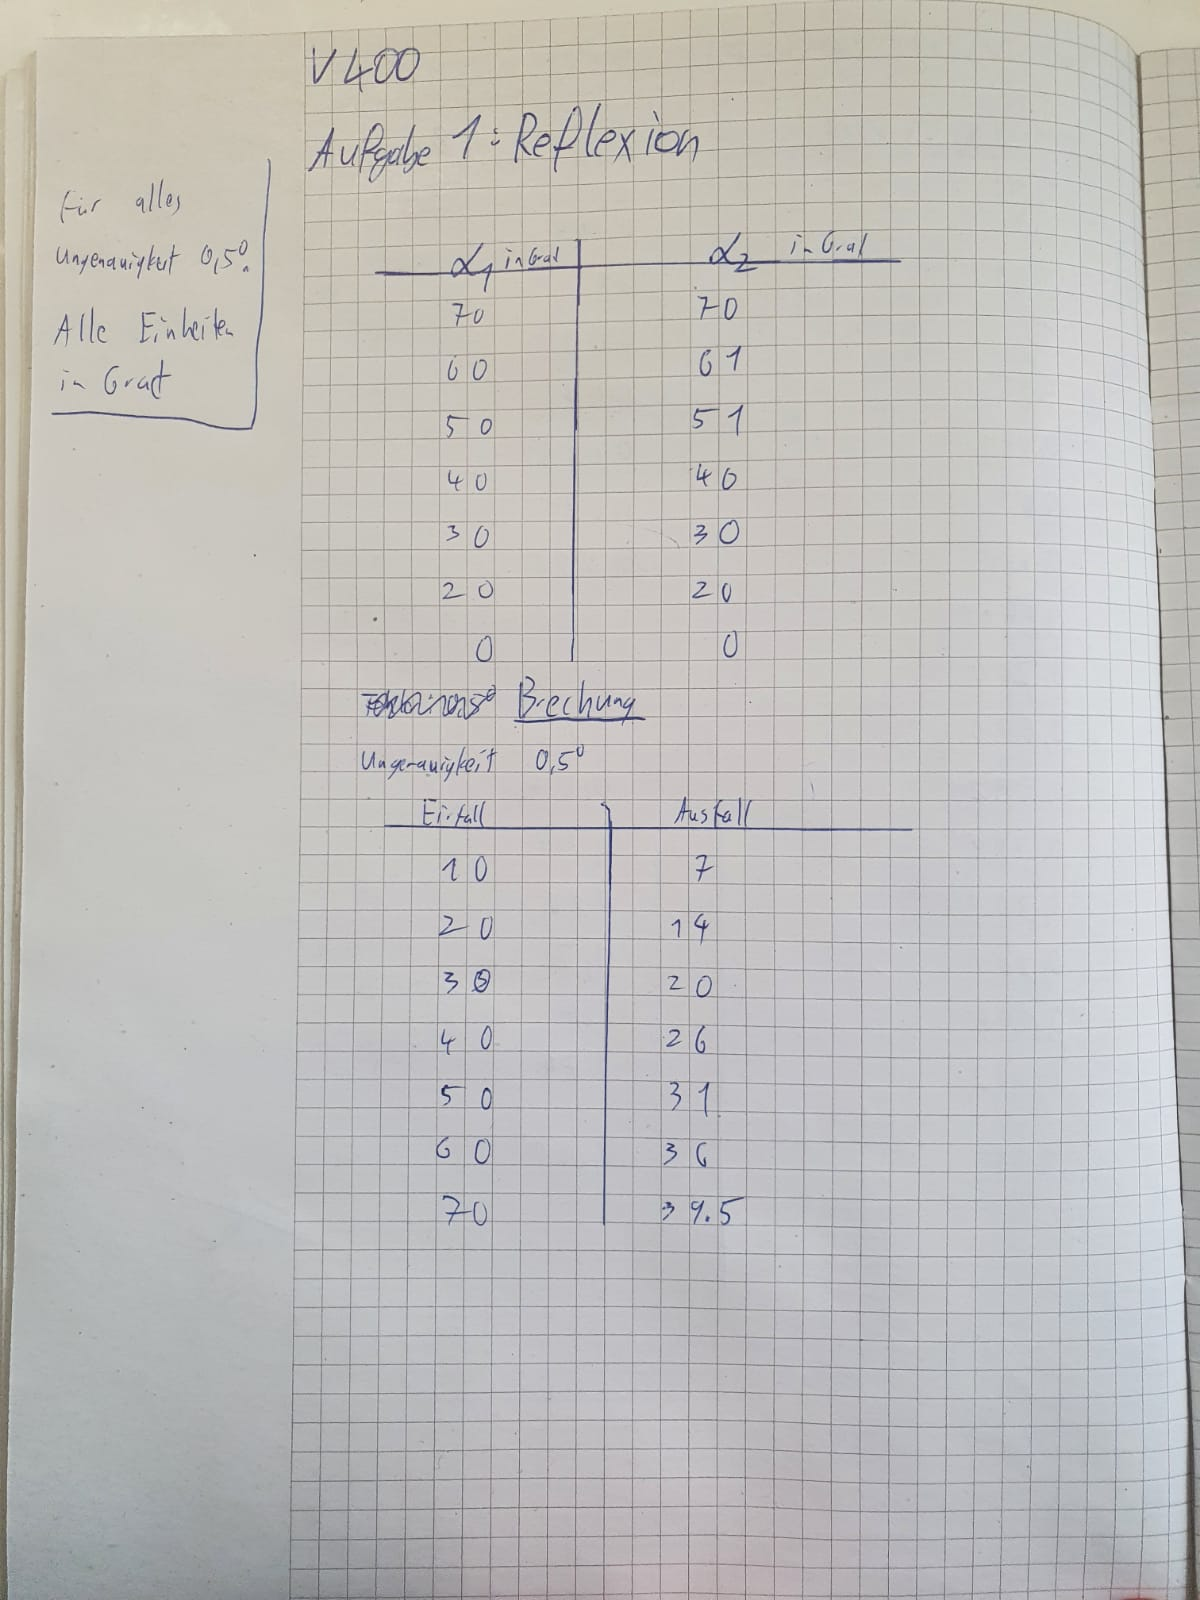
\includegraphics[width=0.63\textwidth]{latex/images/werte1.jpeg}
    \caption{Ein Foto der Messdaten.}
    \label{img:Daten1}
\end{figure}

\begin{figure}[H]
    \centering
    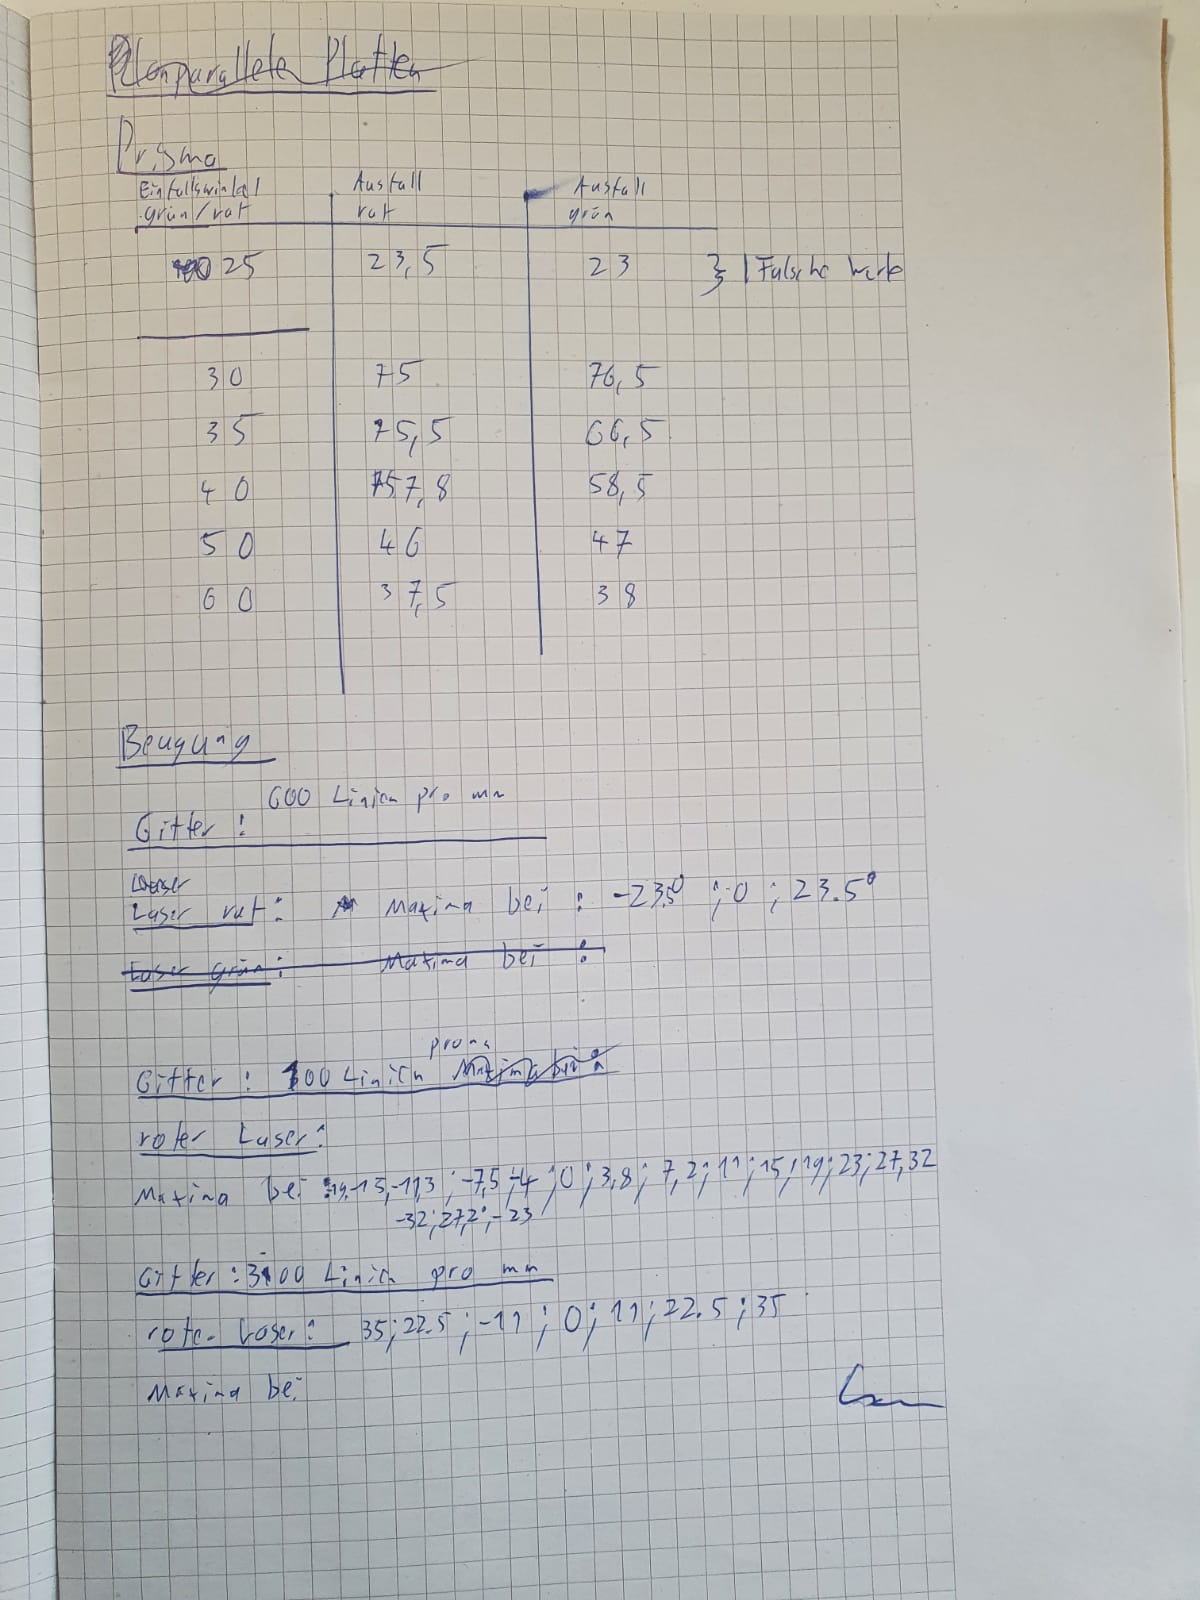
\includegraphics[width=0.63\textwidth]{latex/images/werte2.jpeg}
    \caption{Ein Foto der Messdaten.}
    \label{img:Daten2}
\end{figure}

